\chapter{Introduction}
\label{sec:introduction}

Charge carrier dynamics in an organic semiconductor can often be described in terms of charge hopping between localized states. The hopping rates depend on electronic coupling elements, reorganization energies, and driving forces, which vary as a function of position and orientation of the molecules.  The exact evaluation of these contributions in a molecular assembly is computationally prohibitive. Various, often semi-empirical, approximations are employed instead. The purpose of the toolkit is to simplify the workflow for charge transport simulations, provide a uniform error-control for the methods, flexible platform for their development, and eventually allow in silico pre-screening of organic semiconductors for specific applications. All implemented methods are illustrated by studying charge transport in amorphous films of DCV2T, a thiphene-based organic semiconductor.

\begin{figure*}[t]
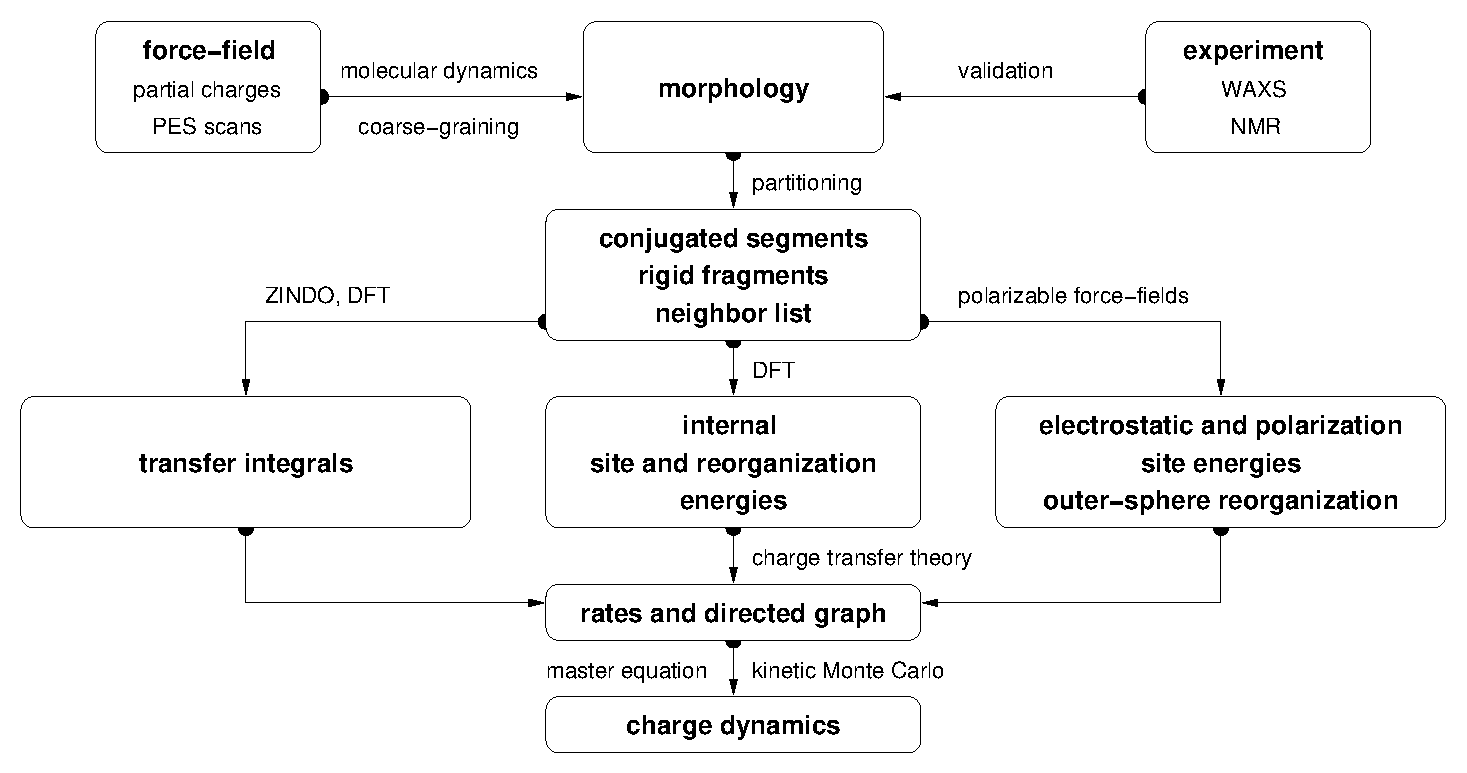
\includegraphics[width=\linewidth]{fig/workflow/workflow}
 \caption{%
   Workflow for microscopic simulations of charge transport.  %
   \label{fig:workflow}}
\end{figure*}

A typical workflow of charge transport simulations is depicted in \fig{workflow}. The first step is the simulation of an atomistic morphology (sec.~\ref{sec:morphology}), which is then partitioned on hopping sites (sec~\ref{sec:conjugated_segments}). The coordinates of the hopping sites are used to construct a list of pairs of molecules (neighbor list). For each pair an electronic coupling element (sec.~\ref{sec:transfer_integrals}), a reorganization energy (sec~\ref{sec:reorganization}), a driving force (sec.~\ref{sec:edisorder}), and eventually the hopping rate are evaluated. The neighbor list and hopping rates define a directed graph. The corresponding master equation is solved using the kinetic Monte Carlo method (sec.~\ref{sec:me}), which allows to explicitly monitor the charge dynamics in the system as well as to calculate time- or ensemble averages of occupation probabilities, charge fluxes, correlation functions, and field-dependent mobilities (sec.~\ref{sec:analysis}).
